%compile: pdflatex path_to_file/project1_report.tex
\documentclass[sigconf]{acmart}
%%
%% \BibTeX command to typeset BibTeX logo in the docs
\AtBeginDocument{%
  \providecommand\BibTeX{{%
    Bib\TeX}}}

%% Rights management information.  This information is sent to you
%% when you complete the rights form.  These commands have SAMPLE
%% values in them; it is your responsibility as an author to replace
%% the commands and values with those provided to you when you
%% complete the rights form.
\setcopyright{acmlicensed}
\copyrightyear{2018}
\acmYear{2018}
\acmDOI{XXXXXXX.XXXXXXX}

%%
%%  Uncomment \acmBooktitle if the title of the proceedings is different
%%  from ``Proceedings of ...''!
%%
%%\acmBooktitle{Woodstock '18: ACM Symposium on Neural Gaze Detection,
%%  June 03--05, 2018, Woodstock, NY}
\acmISBN{978-1-4503-XXXX-X/2018/06}



%%
%% end of the preamble, start of the body of the document source.
\begin{document}

%%
%% The "title" command has an optional parameter,
%% allowing the author to define a "short title" to be used in page headers.
\title{Project 2 - Group 4}

%%
%% The "author" command and its associated commands are used to define
%% the authors and their affiliations.
%% Of note is the shared affiliation of the first two authors, and the
%% "authornote" and "authornotemark" commands
%% used to denote shared contribution to the research.
%The names, student code, and email of each member of the group.

\author{Arda Adali, 0385433}
\affiliation{%
  \institution{Utrecht University}
  \city{Utrecht}
  \country{Netherlands}}
\email{a}

\author{Lena Feiler, 1751611}
\affiliation{%
  \institution{Utrecht University}
  \city{Utrecht}
  \country{Netherlands}}
\email{l.l.feiler@students.uu.nl}

\author{Kerem Dogan, 1696637}
\affiliation{%
  \institution{Utrecht University}
  \city{Utrecht}
  \country{Netherlands}}
\email{a}

\author{Sofia Bianchini, 7273746}
\affiliation{%
  \institution{Utrecht University}
  \city{Utrecht}
  \country{Netherlands}}
\email{a}


%%
%% By default, the full list of authors will be used in the page
%% headers. Often, this list is too long, and will overlap
%% other information printed in the page headers. This command allows
%% the author to define a more concise list
%% of authors' names for this purpose.
\renewcommand{\shortauthors}{Trovato et al.}

%%
%% The abstract is a short summary of the work to be presented in the
%% article.
\begin{abstract}
  A short summary of the report (no more than 100 words). The abstract
should include a concise overview of the context of the report (what the report
is about and what it describes), of the results obtained from the peer assessment
(Project 2 Part 2), and of the key insights gained from the assessment.
\end{abstract}


\ccsdesc[500]{Do Not Use This Code~Generate the Correct Terms for Your Paper}
\ccsdesc[300]{Do Not Use This Code~Generate the Correct Terms for Your Paper}
\ccsdesc{Do Not Use This Code~Generate the Correct Terms for Your Paper}
\ccsdesc[100]{Do Not Use This Code~Generate the Correct Terms for Your Paper}

%%
%% Keywords. The author(s) should pick words that accurately describe
%% the work being presented. Separate the keywords with commas.
\keywords{Do, Not, Us, This, Code, Put, the, Correct, Terms, for,
  Your, Paper}
%% A "teaser" image appears between the author and affiliation
%% information and the body of the document, and typically spans the
%% page.
\begin{teaserfigure}
  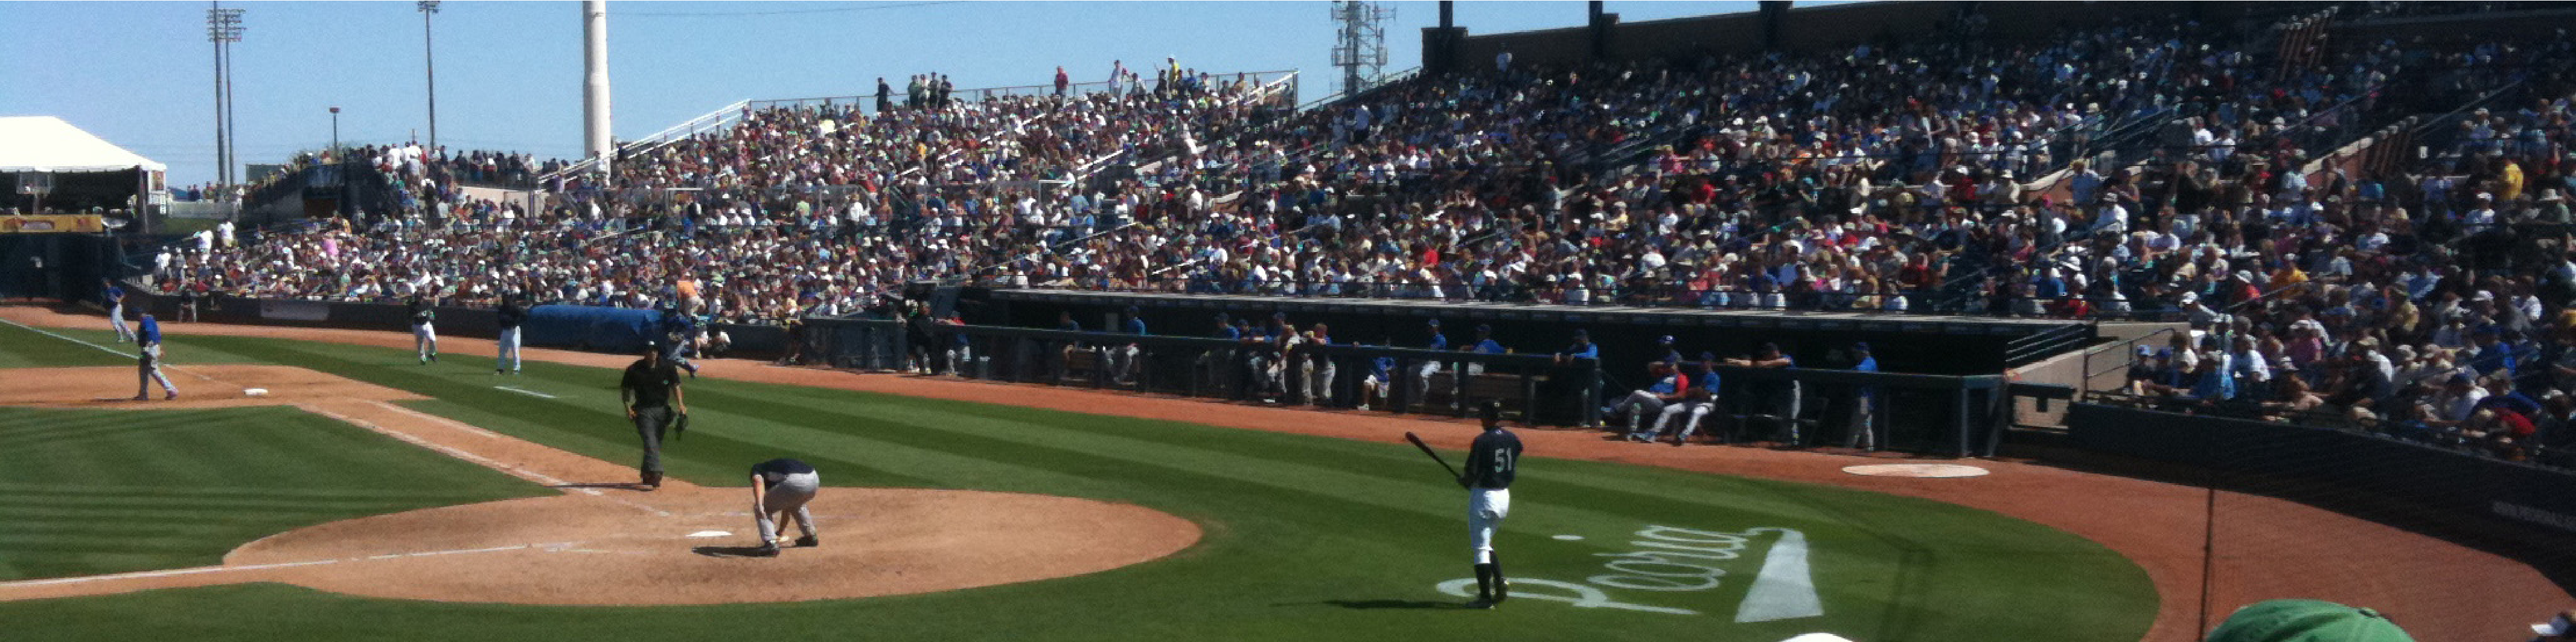
\includegraphics[width=\textwidth]{sampleteaser}
  \caption{Seattle Mariners at Spring Training, 2010.}
  \Description{Enjoying the baseball game from the third-base
  seats. Ichiro Suzuki preparing to bat.}
  \label{fig:teaser}
\end{teaserfigure}

\received{02 April 2025}

\maketitle

\section{Introduction}
A short introduction section, which briefly introduces the report and
its sections.


\section{Algorithm for Generating Natural Language Explanations}
A section describing
the algorithm implemented for generating natural language explanations
of an action starting from an execution trace (as per Section 3.1). The description
should explain how the algorithm works and it should include and refer to the
pseudocode of the algorithm, which should be written using the Latex algorithm environment.
The pseudocode of the main body of the algorithm should be included
directly inline as part of the section. If additional algorithms (e.g., sub-functions,
etc.) are used and are necessary to be explained in order to fully understand the
main algorithm, these should also be included in the report in appendix A (which
does not count on the total number of pages). The use of appendix, however, should
be minimized, and unnecessarily excessive use of appendix will be graded negatively.


\section{Experiments}
A section describing the experiment conducted with peer students (as
per Section 3.2) to evaluate the output of the algorithm. The report should describe
the data that was given to the other students, a description of the questions that were
asked to peers to evaluate the algorithm (including a motivation for the questions in
terms of which human criteria of good explanations they refer to), and a reflection
on the results obtained. The results should include: the number of peer feedback
obtained, both a table and a likert plot reporting the answers of the feedback to the
likert questions, and a discussion of the results and the feedback in reference to the
algorithm developed.

\section{Conclusion}
A short conclusion section that wraps up the document and summarizes
what has been presented and the main insights.

%%
%% The acknowledgments section is defined using the "acks" environment
%% (and NOT an unnumbered section). This ensures the proper
%% identification of the section in the article metadata, and the
%% consistent spelling of the heading.
\begin{acks}
To Robert, for the bagels and explaining CMYK and color spaces.
\end{acks}

%%
%% The next two lines define the bibliography style to be used, and
%% the bibliography file.
\bibliographystyle{ACM-Reference-Format}
\bibliography{sample-base}


\end{document}
\endinput
